

The study of neutrino oscillations is today focused on the determination of the remaining unknowns in the three flavor framework,
namely the CP-violating phase $\delta_{\rm CP}$, the deviation of the $\theta_{23}$ angle from $\pi$/4 (also called the octant determination), and the mass ordering. This can be done by the long baseline experiments. Another important task is the high precision determination of all the mass and mixing parameters. For a recent review on the subject refer to \cite{Giganti:2017fhf}. 

The long baseline oscillation experiments will precisely measure the neutrino oscillation probability beyond the leading order term, for a beam of muon neutrinos.
\newpage
The probability of electron neutrino appearance in a beam of muon neutrinos is given by:
\begin{eqnarray}
P(\nu_{\mu} \rightarrow \nu_e) & = & \sin^2 \theta_{23} \frac{\sin^2 2 \theta_{13}}{(A-1)^2} \sin^2 [(A-1) \Delta_{31}] \nonumber \\
&+& \alpha^2 \cos^2 \theta_{23} \frac{\sin^2 2 \theta_{12}}{A^2} \sin^2 (A\Delta_{31}) \nonumber \\
&-& \alpha \frac{\sin 2 \theta_{12}\sin 2 \theta_{13}\sin 2 \theta_{23}\cos  \theta_{13}\sin  \delta_{CP}}{A (1-A)} \sin \Delta_{31} \sin (A\Delta_{31})\sin[ (1-A) \Delta_{31}] \nonumber \\
&+& \alpha \frac{\sin 2 \theta_{12}\sin 2 \theta_{13}\sin 2 \theta_{23}\cos  \theta_{13}\cos  \delta_{CP}}{A (1-A)} \cos \Delta_{31} \sin (A\Delta_{31})\sin[ (1-A) \Delta_{31}] \nonumber\\
\label{eq:theta13app}
\end{eqnarray}
where $ \alpha = \Delta m^2_{21} / \Delta m^2_{31}$, $\Delta_{ji}= \Delta m^2_{ji} L / 4 E$ and $A= 2\sqrt 2 G_F n_e E/ \Delta m^2_{31}$.
The corresponding formula for $P(\bar \nu_{\mu} \rightarrow \bar \nu_e)$ can be obtained by reversing the signs of the terms proportional to $\sin \delta_{CP}$ and to $A$. The different terms contributing to $P(\nu_{\mu} \rightarrow \nu_e)$,  are plotted in Fig.~\ref{fig:t2kappprob} together with the total contribution from matter effects, assuming a baseline of 295 km.

\begin{figure} [htbp!]
\begin{center}
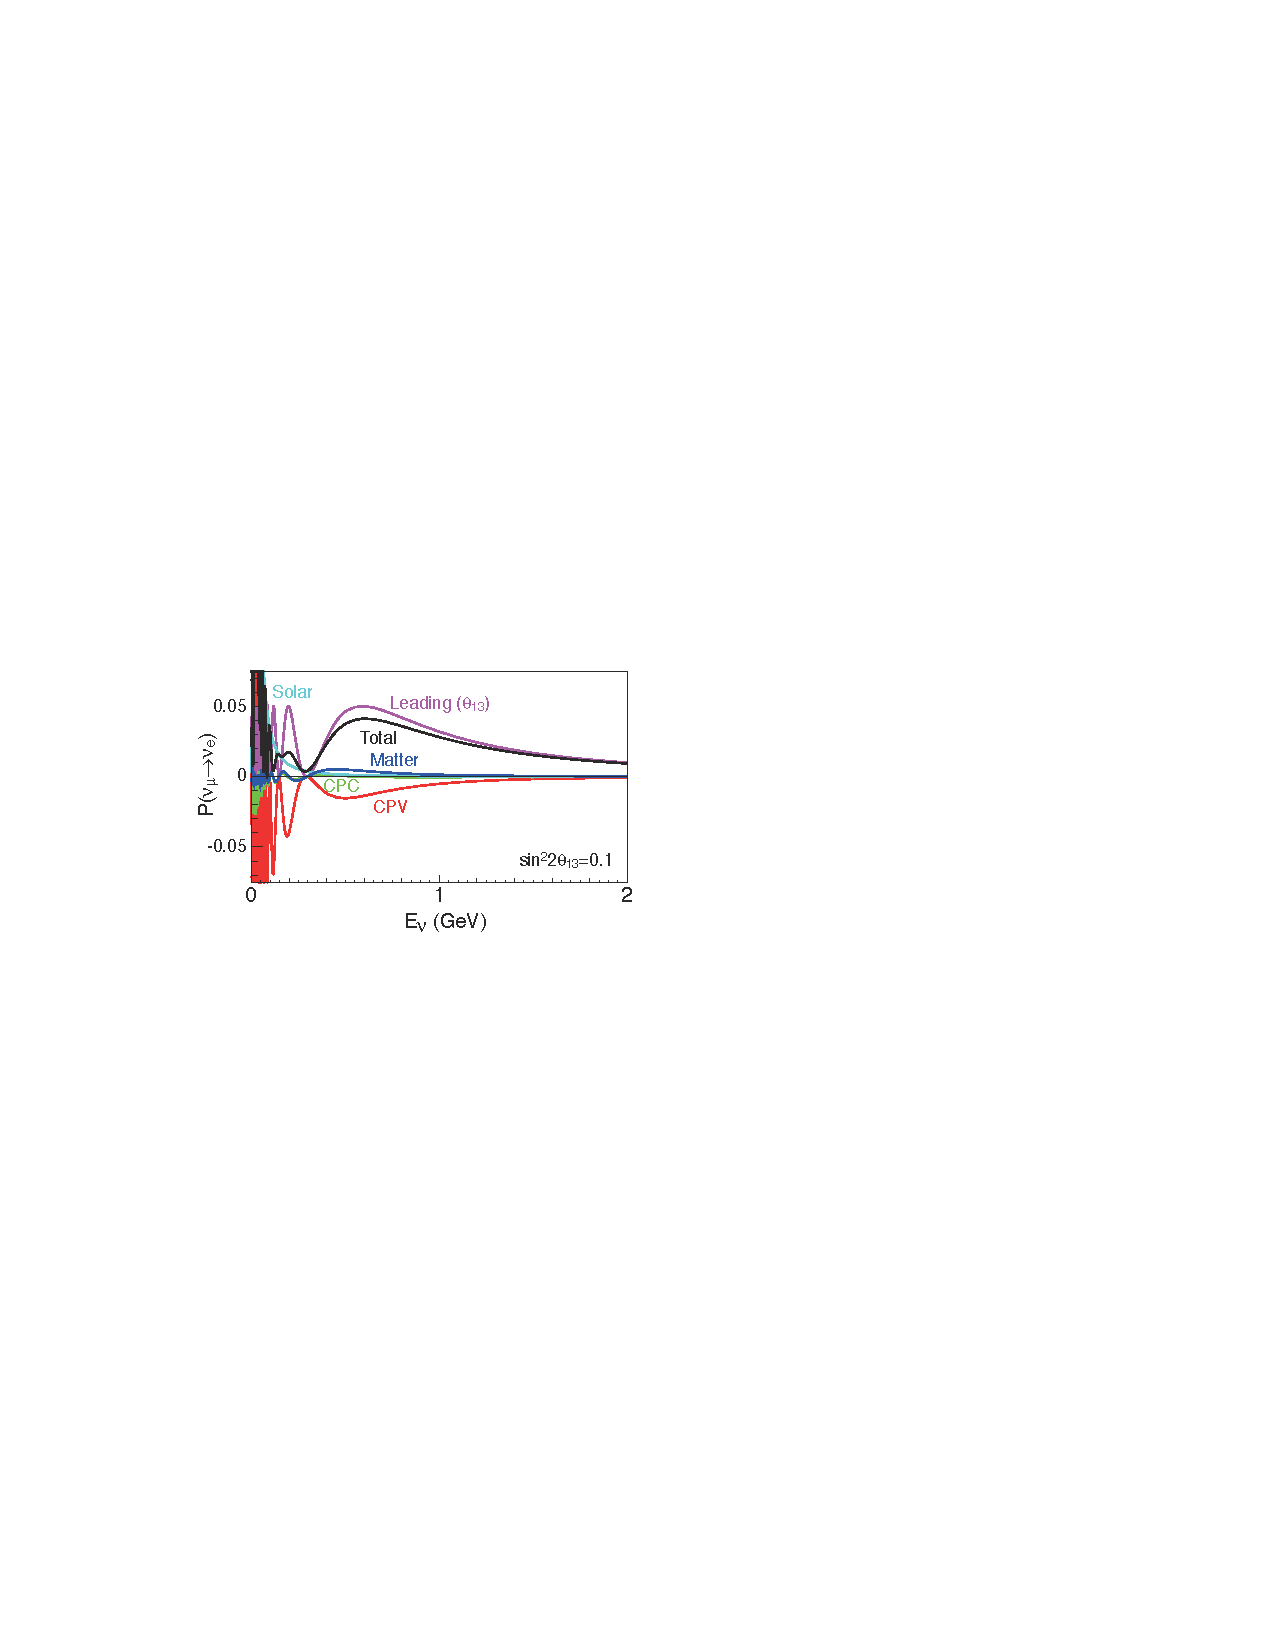
\includegraphics[width=10cm]{\main/Neutrino/img/papp_prob_2.pdf}
\caption{\label{fig:t2kappprob} Oscillation probability $\nu_\mu \rightarrow \nu_e$ as a function of neutrino energy with L = 295 km, ${\sin}^2(2\theta_{13})$ = 0.1, $\delta_{CP}$= $\pi/2$ and normal mass ordering. The contribution of each term in the oscillation probability~Eq.~(\ref{eq:theta13app}) is shown separately. The first term in that equation is shown by the curve labeled "Leading", the second term is labeled "Solar" (so called because $\theta_{12}$ governs the oscillation of solar neutrinos), the third CP-violating term (CPV) proportional to $\sin \delta_{CP}$ is labeled CPV. The fourth CP-conserving (CPC) term proportional to $\cos \delta_{CP}$ is labeled CPC.}
\end{center}
\end{figure}

The first term in Eq.~(\ref{eq:theta13app}) (labelled "leading" in Fig.~\ref{fig:t2kappprob}) is the leading order term and corresponds to the 1-3 sector oscillations driven by the squared-mass difference $\Delta m^2_{31}$. %It should be noticed that it contains also a factor $\sin^2 \theta_{23}$ that is sensitive to the octant of $\theta_{23}$.
%
%The second term (labelled "solar" in Fig.~\ref{fig:t2kappprob}) corresponds to the 1-2 sector oscillations and is suppressed because of the smallness of $ \alpha \simeq 0.03$. 
%
The third term ("CPV") contains the CP-violating part. % and is proportional to the Jarlskog invariant $J$, 
%proportional to the sinus of the three mixing angles.
%$J=C^2_{13}C_{12}C_{23}S_{12}S_{13}S_{23} \sin \dcp $. 
It modifies the leading order term by as much as $\pm$ 30 \% for $\delta_{CP} = \mp \pi/2$, respectively, in the case of neutrinos.
%
%The fourth term ("CPC") is CP conserving, as it is proportional to $\cos \delta_{CP}$. Since its dependence on $\delta_{CP}$ is different from the one of the third term, it might be useful for resolving degeneracies. As this term is proportional to $\cos \Delta_{31}$, it is zero at the first vacuum oscillation maximum, $\Delta_{31}=\pi/2$. It must therefore be studied for L/E away from the first oscillation maximum. 
%
Matter effects enter through the $A$ term proportional to the ratio $E/E_{res}$, where $E_{res}$ is the energy for which the resonance condition is attained in the medium of constant density. Since the resonance condition can be satisfied either for neutrinos or for antineutrinos, depending on the sign of $\Delta m^2_{31}$ and therefore on the mass ordering, matter effects either enhance $ P (\nu_\mu \rightarrow \nu_e)$ or  $ P (\bar{\nu}_\mu \rightarrow \bar{\nu}_e)$.
The $A$ term is approximately 5\% for T2K and Hyper-Kamiokande, about 20\% for DUNE.

In principle the precise measurement of $P(\nu_{\mu} \rightarrow \nu_e)$ and $P(\bar{\nu}_{\mu} \rightarrow \bar{\nu}_e)$ allows by itself to determine all the remaining unknowns among the the neutrino mixing parameters: as long baseline experiments based on rather pure muon neutrino (or muon antineutrino) beams allow to conduct this measurement with  well-defined experimental conditions, they have received a lot of attention and are today the central focus of the experimental effort. Today they are a strategic scientific priority for the international community and will continue to be for the next two decades.

While multiple ambiguities could play a role in the extraction of physics parameters from the observables, in practice the impact of these ambiguities will be greatly mitigated by two facts. First, reactor neutrino experiments have provided a clean and high precision measurements of $\theta_{13}$. Second, present and future experiments will provide measurements at different baselines, and therefore with different strength of the matter effects, going from the shorter baseline of T2K and Hyper-Kamiokande (295 km) to the longer baseline of NOVA (810 km) and DUNE (1300 km). This will help decorrelate the effect of CP violation from matter effects.
%(Fig.~\ref{fig:novaellipse}).

%\begin{figure} [htbp!]
%\begin{center}
%add plot!!!
%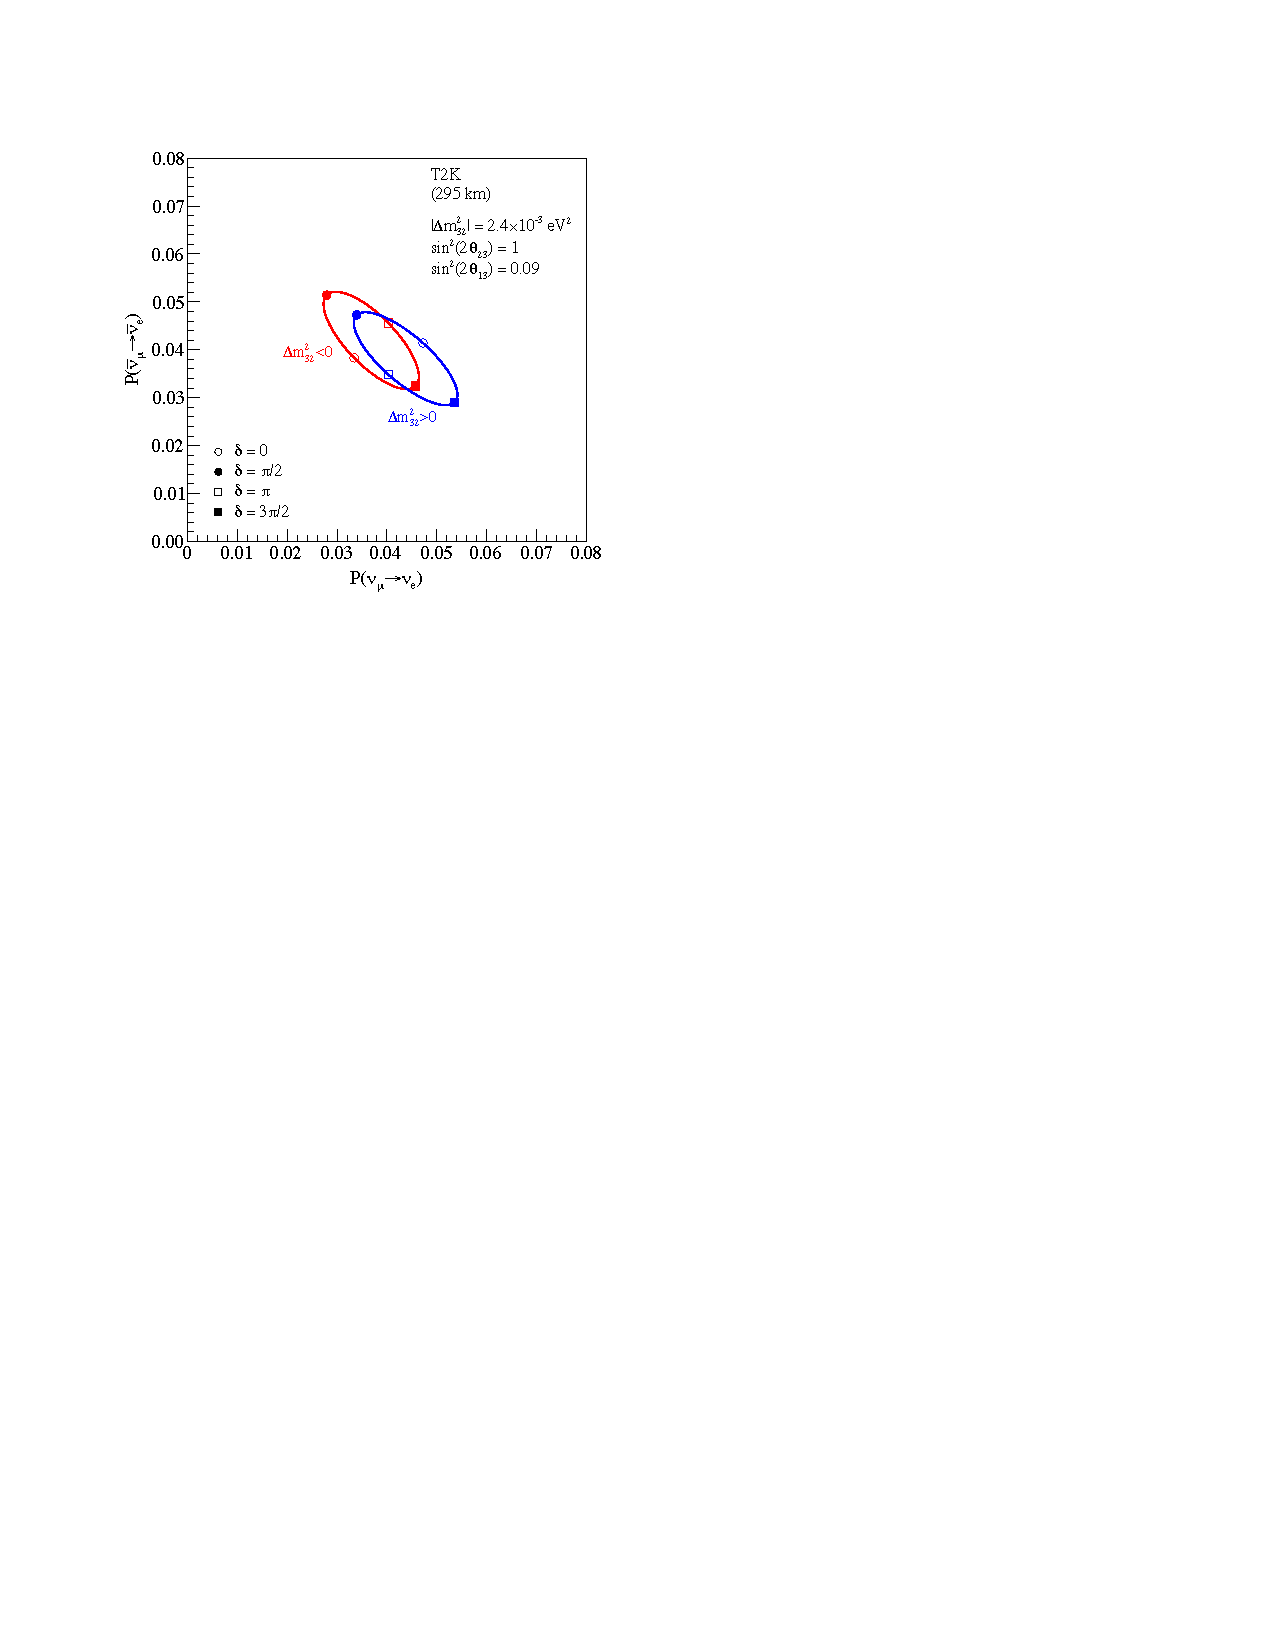
\includegraphics[scale=0.6]{\main/Neutrino/img/t2k_ellipse.pdf}
%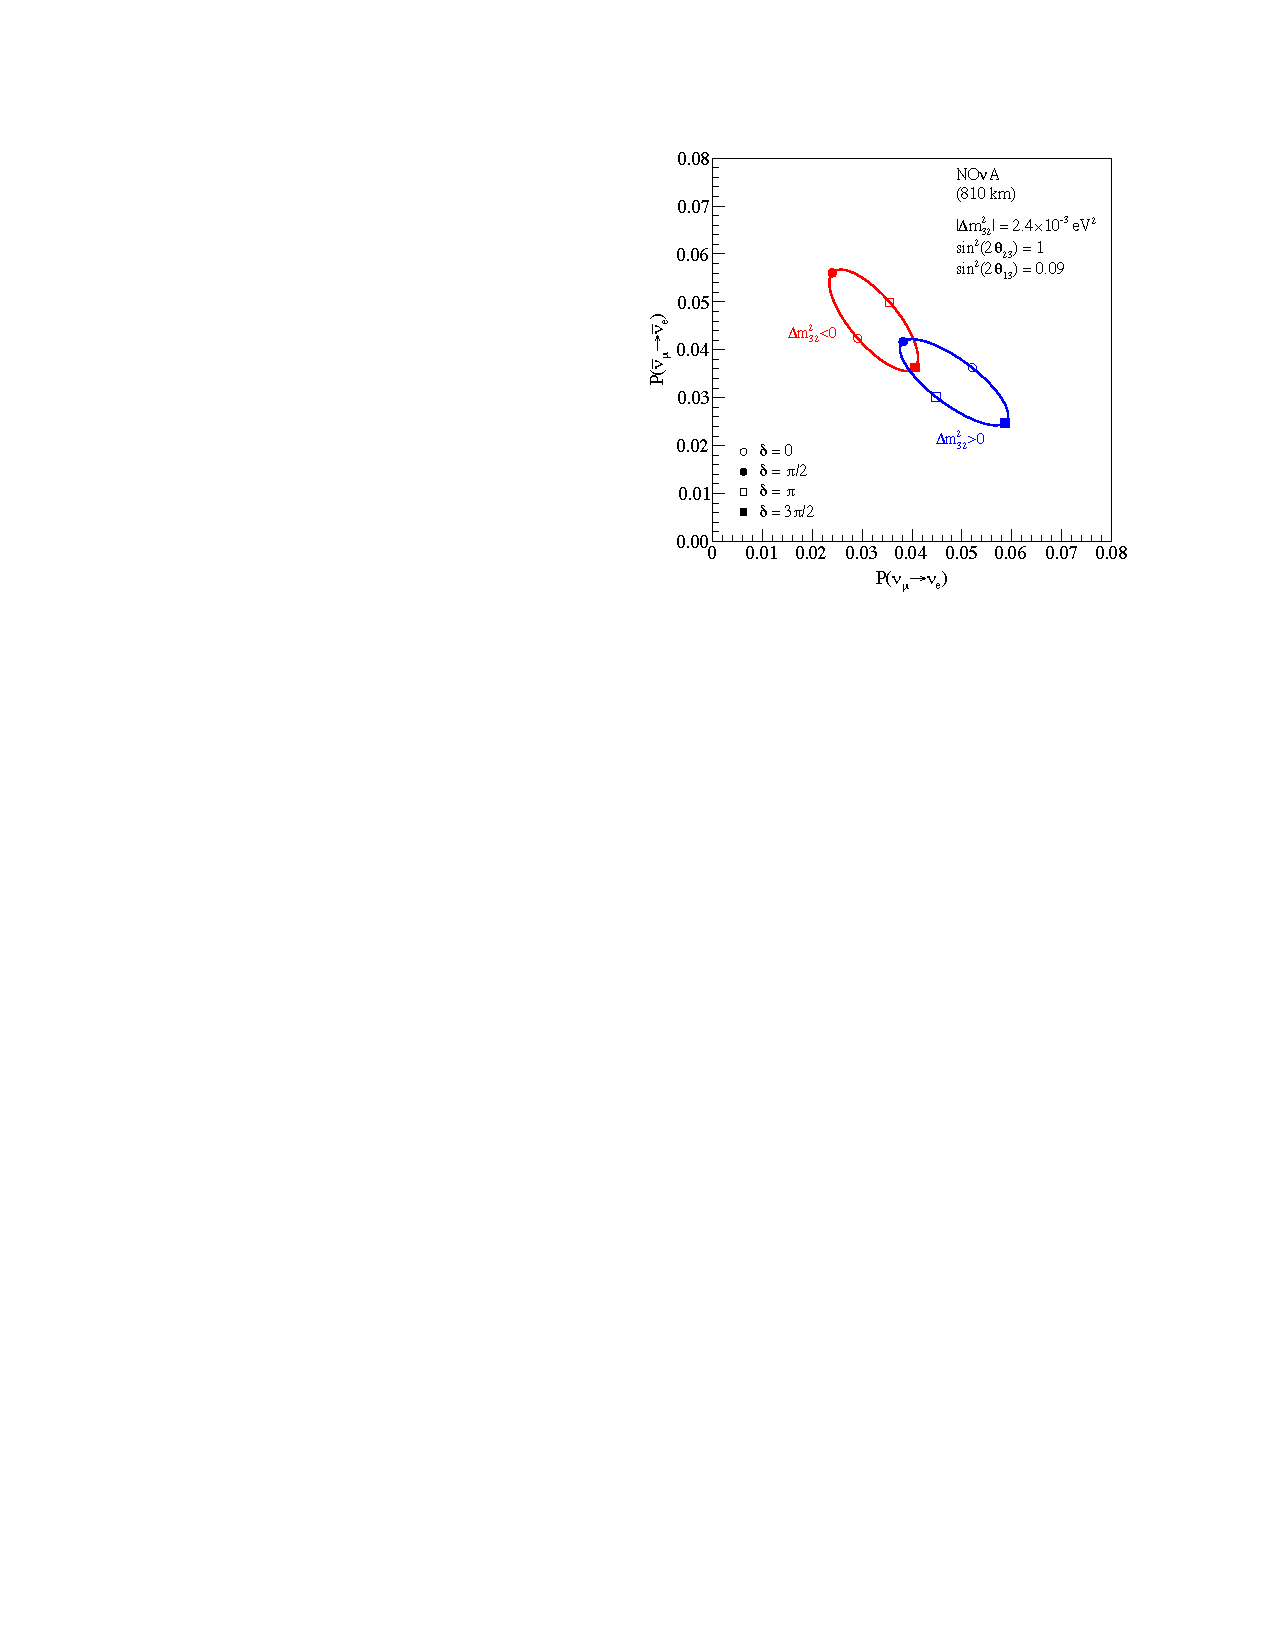
\includegraphics[scale=0.6]{\main/Neutrino/img/nova_ellipse.pdf}
%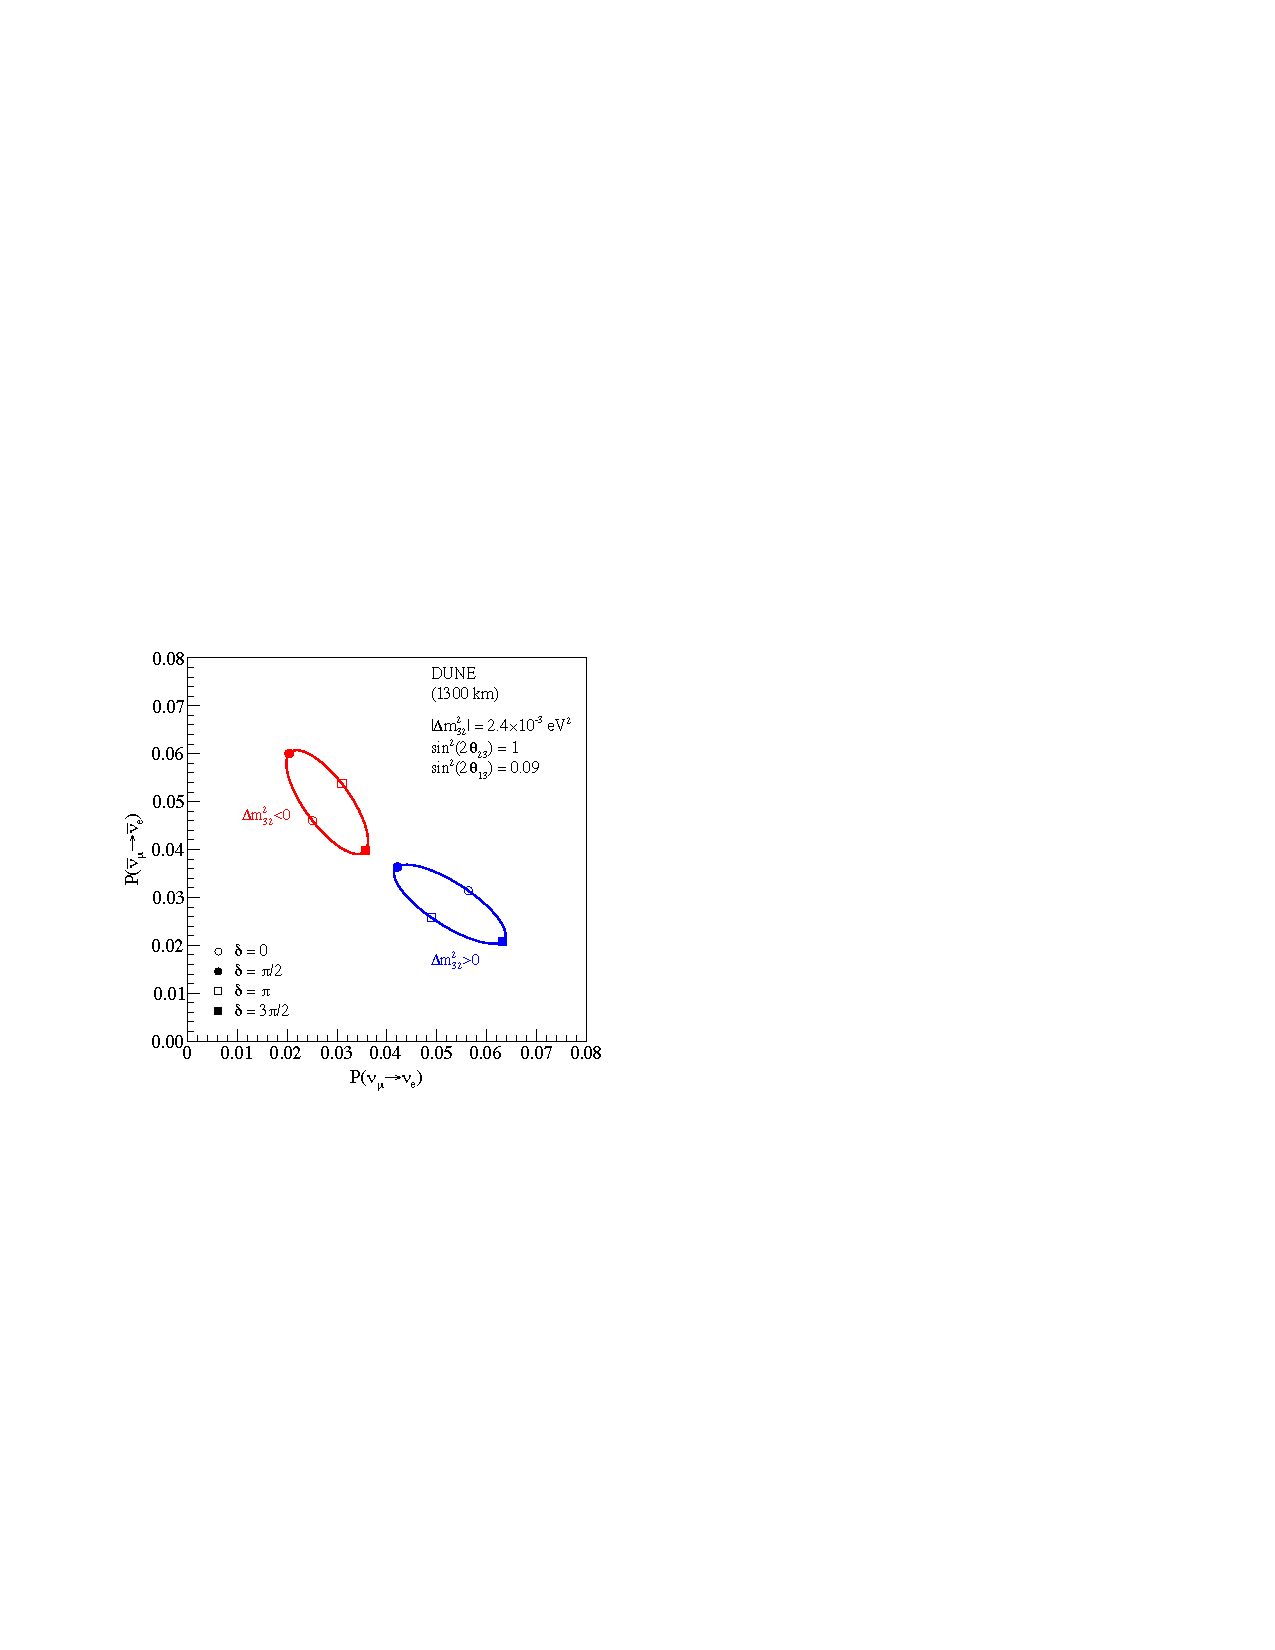
\includegraphics[scale=0.6]{\main/Neutrino/img/dune_ellipse.pdf}
%\caption{\label{fig:novaellipse} Oscillation probabilities $ P (\nu_\mu \rightarrow \nu_e)$ and $ P (\bar{\nu}_\mu \rightarrow \bar{\nu}_e)$ for normal (blue) and inverted (red) mass ordering, assuming T2K (left), NOVA (center) and DUNE (right) baselines and a representative L/E value of 0.4 km/MeV~\cite{Patterson:2015xja}. 
%}
%\end{center}
%\label{fig:biprob}
%\end{figure}


\subsection{The present experiments T2K and NOVA}

The presently running experiments T2K in Japan and NOVA in USA will continue to produce world-leading results in the coming years. As reported above, in conjunction with other measurements, the data from these experiments already today provides an indication favouring the normal ordering at the 3 $\sigma$ level, and a weak hint of CP violation in neutrino oscillation. % at the 2 $\sigma$ level.

The J-PARC main ring, presently operating at 485 kW beam power for the T2K neutrino beam line is currently undergoing a series of upgrades allowing it to reach 1 MW around 2022 and later 1.3 MW in the Hyper-Kamiokande era [ID158]. %\cite{lodovico-esppu}. 
%The T2K experiment uses the 50 kt water Cherenkov detector Super-Kamiokande as its far detector. 
The T2K Collaboration has submitted a proposal for an extension of T2K running (T2K-II) accumulating 20$\times$10$^{21}$ protons-on-target (POT), that is 6 times the present exposure.
This aims at an initial observation of the $\delta_{CP}$ parameter at the 3\,$\sigma$ level for a significant range of the possible values (Fig.~\ref{fig:t2k2sensi}) by 2026. T2K has also launched an upgrade of its near detector complex~\cite{Abe:2019whr} in order to reduce the systematic uncertainties to match this increase of the data sample. %T2K will also benefit from the Gadolinium loading in the water of the Super-Kamiokande detector, presently serving also as the far detector of T2K. Gadolinium will enhance neutron tagging and therefore the CP violation measurement. 

\begin{figure} [htbp!]
\begin{center}
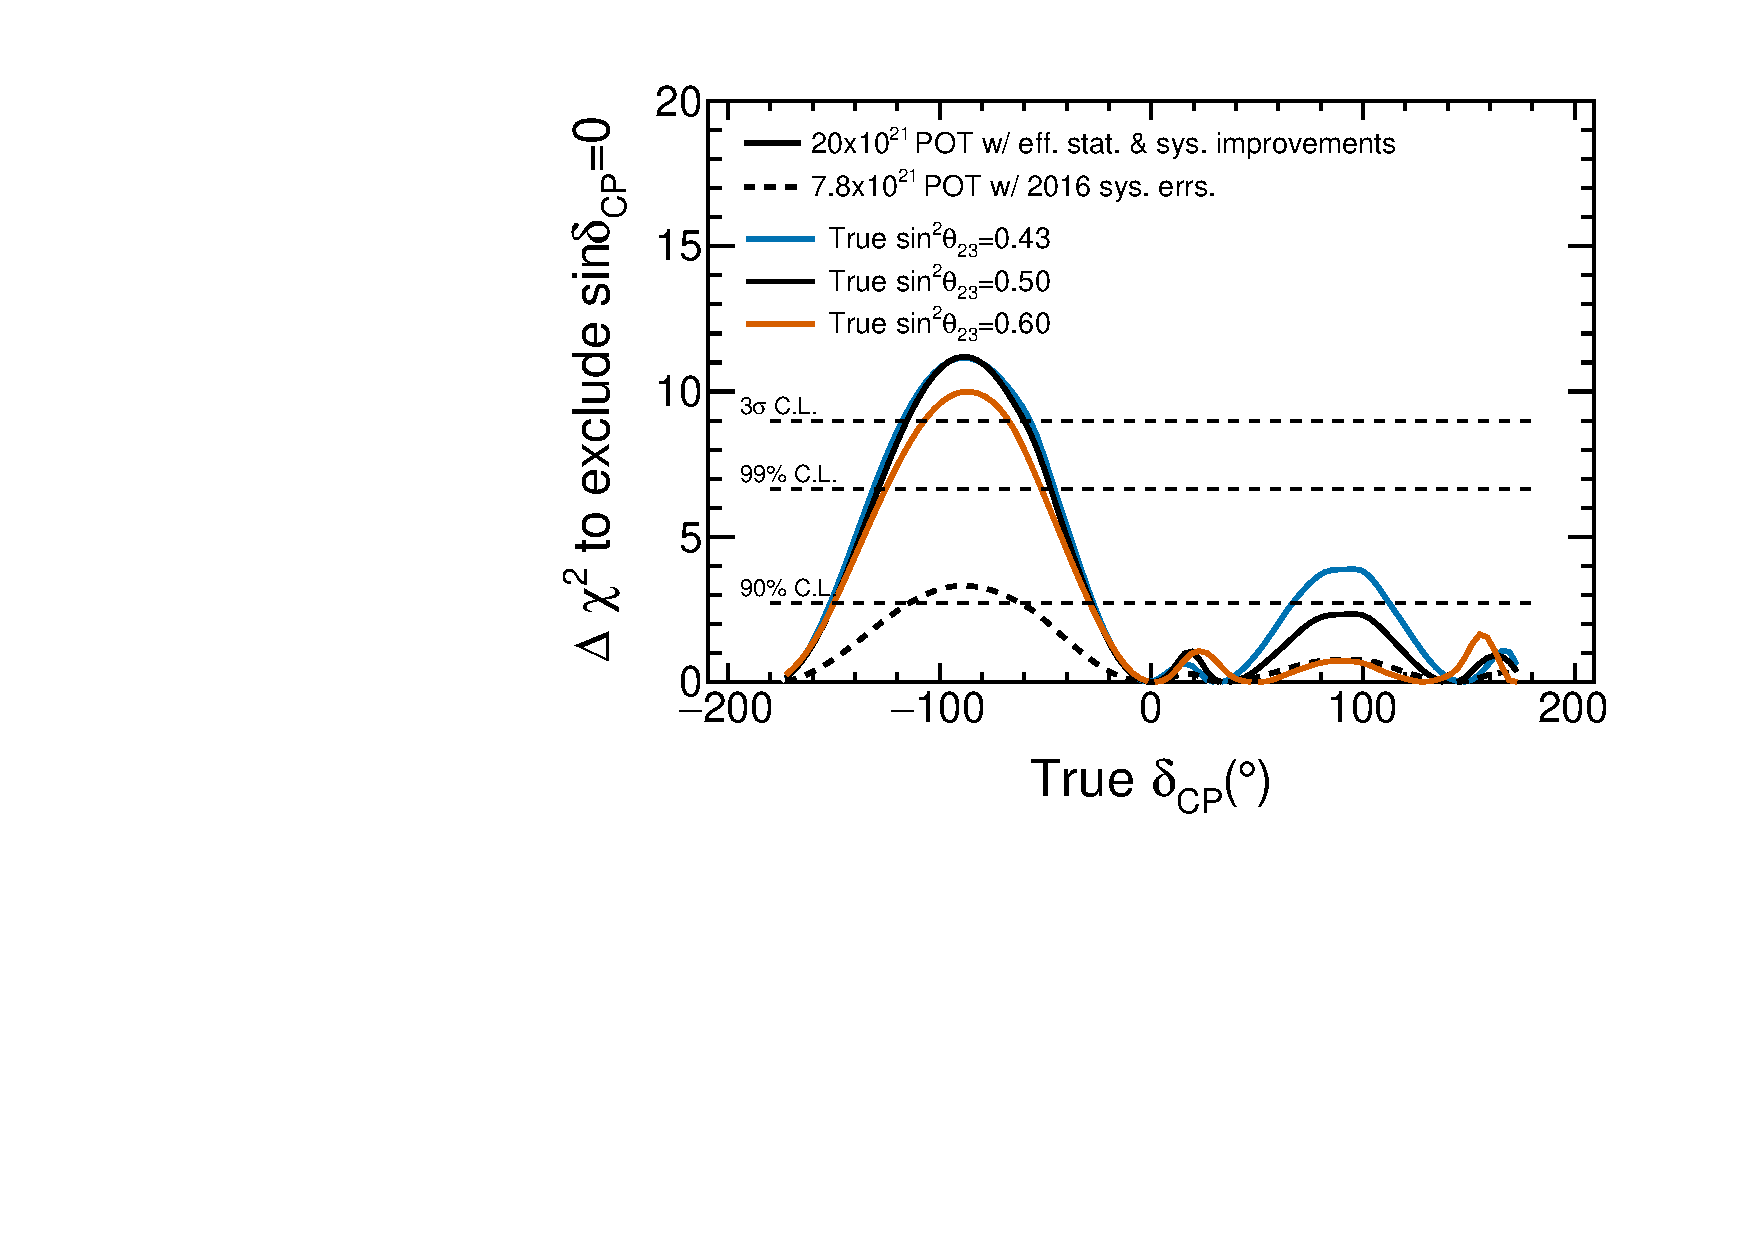
\includegraphics[scale=0.35]{\main/Neutrino/img/t2kpre_dcp_point1_100k4check_100ksensi_wreactorthrow_optv2s13off_truedcp_unknownMH_fakesyst_lohidcpExclusive.pdf}
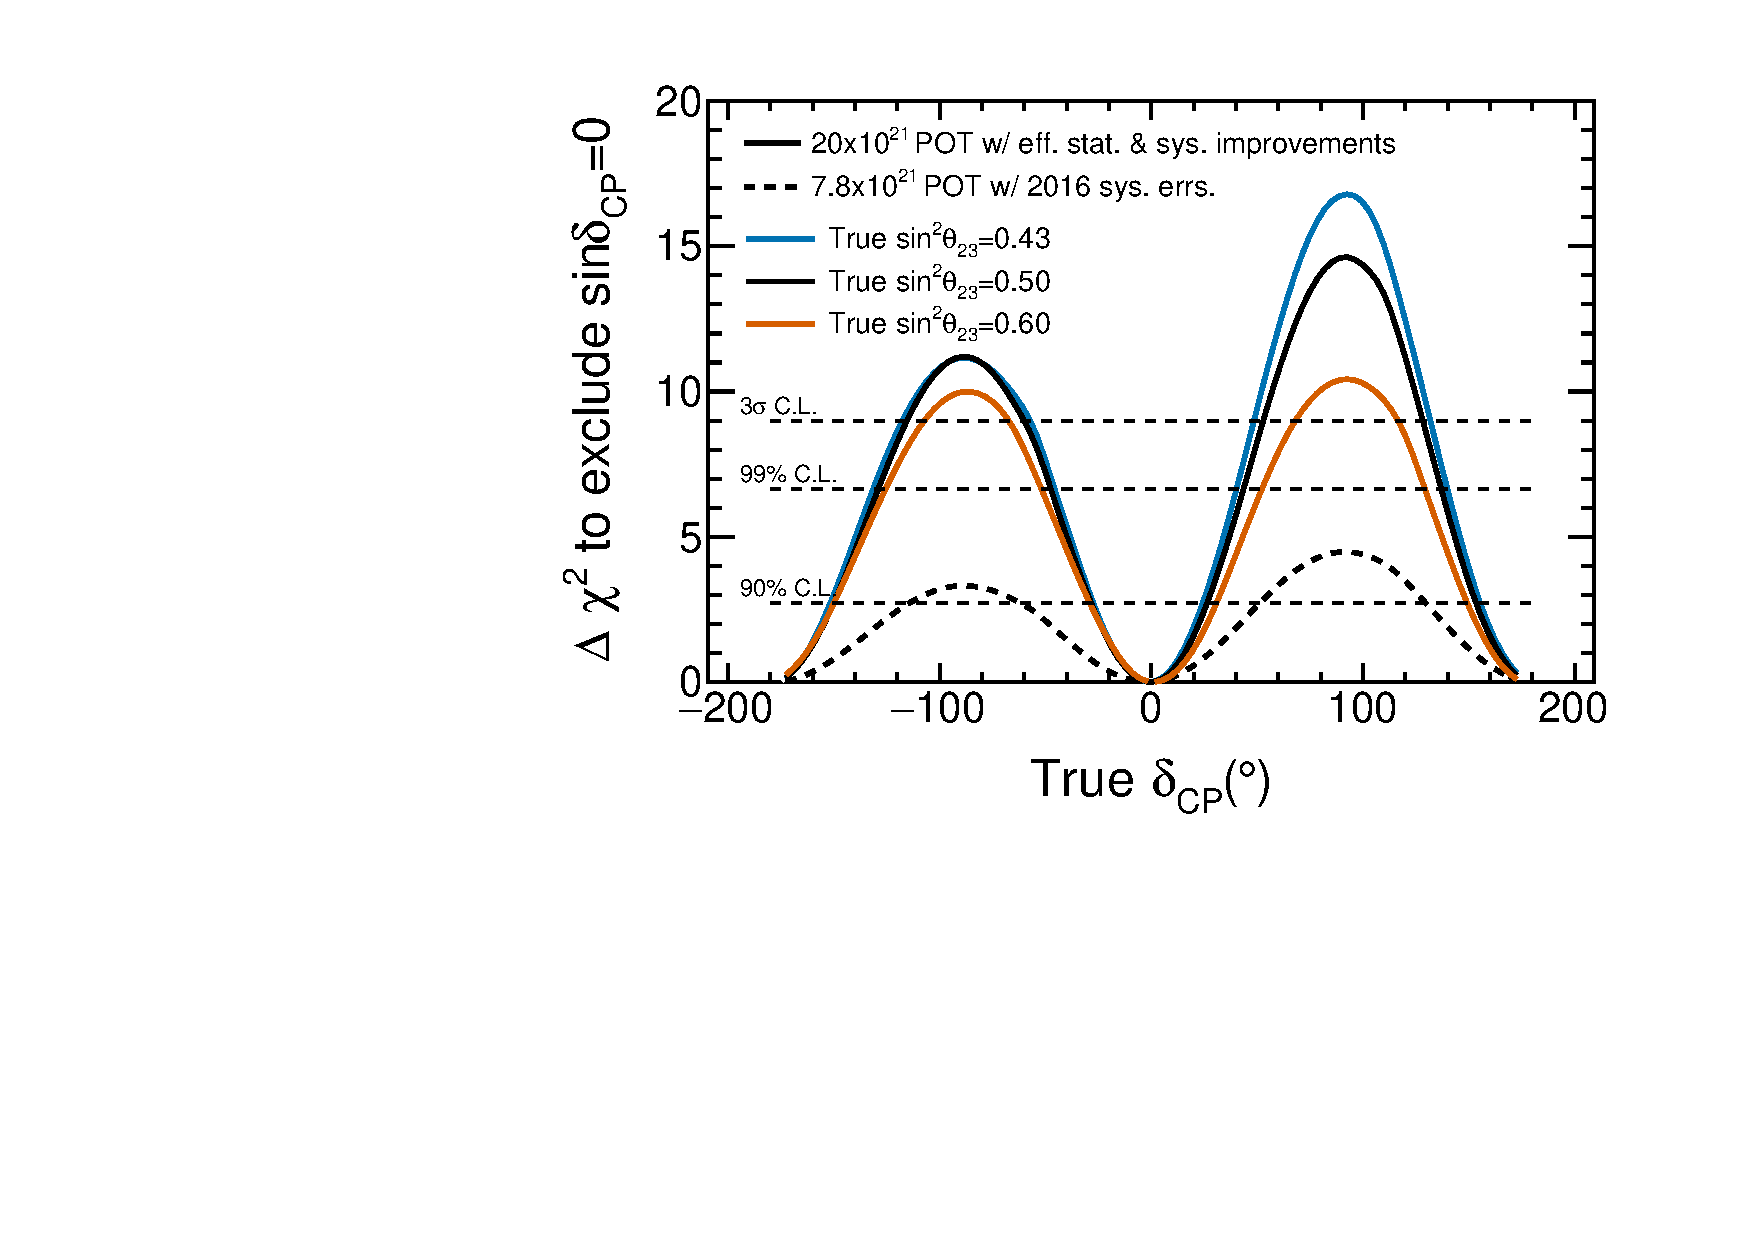
\includegraphics[scale=0.35]{\main/Neutrino/img/t2kpre_dcp_point1_100k4check_100ksensi_wreactorthrow_optv2s13off_truedcp_fakesyst_lohidcpExclusive.pdf}
\caption{\label{fig:t2k2sensi} Sensitivity to CP violation as a function of the true
$\delta_{CP}$ for three values of $\sin^2 (2 \theta_{23})$ (0.43, 0.50, 0.60) and normal ordering, for the full T2K-II exposure of $20\times 10^{21}$ POT and a reduction of the systematic error to 2/3 of the 2016 T2K uncertainties. On the left plot the mass ordering is considered unknown, while on the right plot it is considered known~\cite{Abe:2016tez}.}
\end{center}
\end{figure}


NOVA [ID167] %\cite{fnal-esppu} 
is based on the NuMI beamline operating at 700 kW, with opportunities to increase to 900 kW by 2021. The NOVA far detector is a 14 kt liquid scintillator calorimeter located in Ash River, at 810 km from the neutrino source. With its longer baseline NOVA has interesting sensitivity to the mass ordering. For the currently favoured set of oscillation parameters, NOVA has potential sensitivity to the mass ordering at 3 $\sigma$ in 2020, and similar sensitivity to CP violation by 2024. % (Fig.~\ref{fig:novasensidcp}). 

%\begin{figure}[htbp]
%\begin{minipage}[c]{.46\linewidth}
%   	      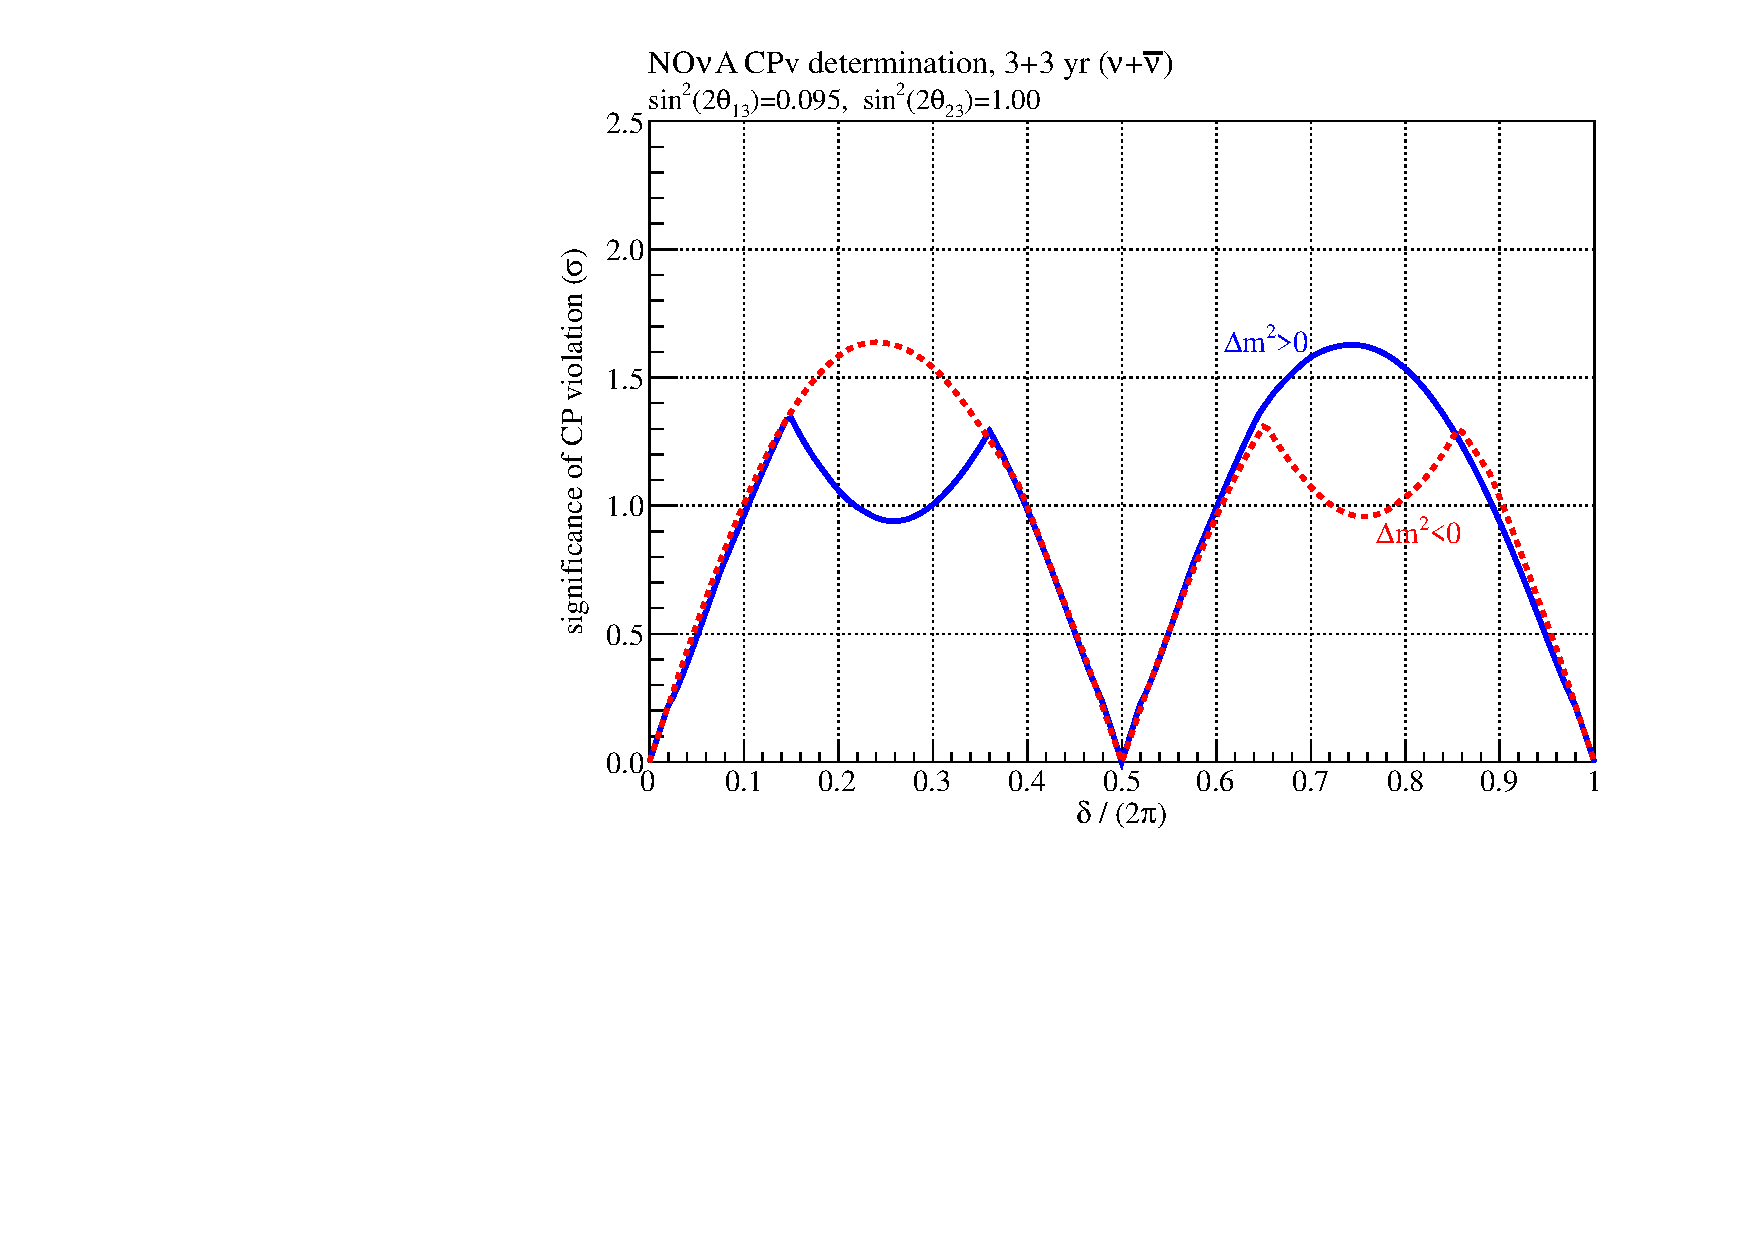
\includegraphics[width=0.9\linewidth]{\main/Neutrino/img/30_CPSignificance.pdf}
%   \end{minipage} \hfill
%   \begin{minipage}{.46\linewidth}
%      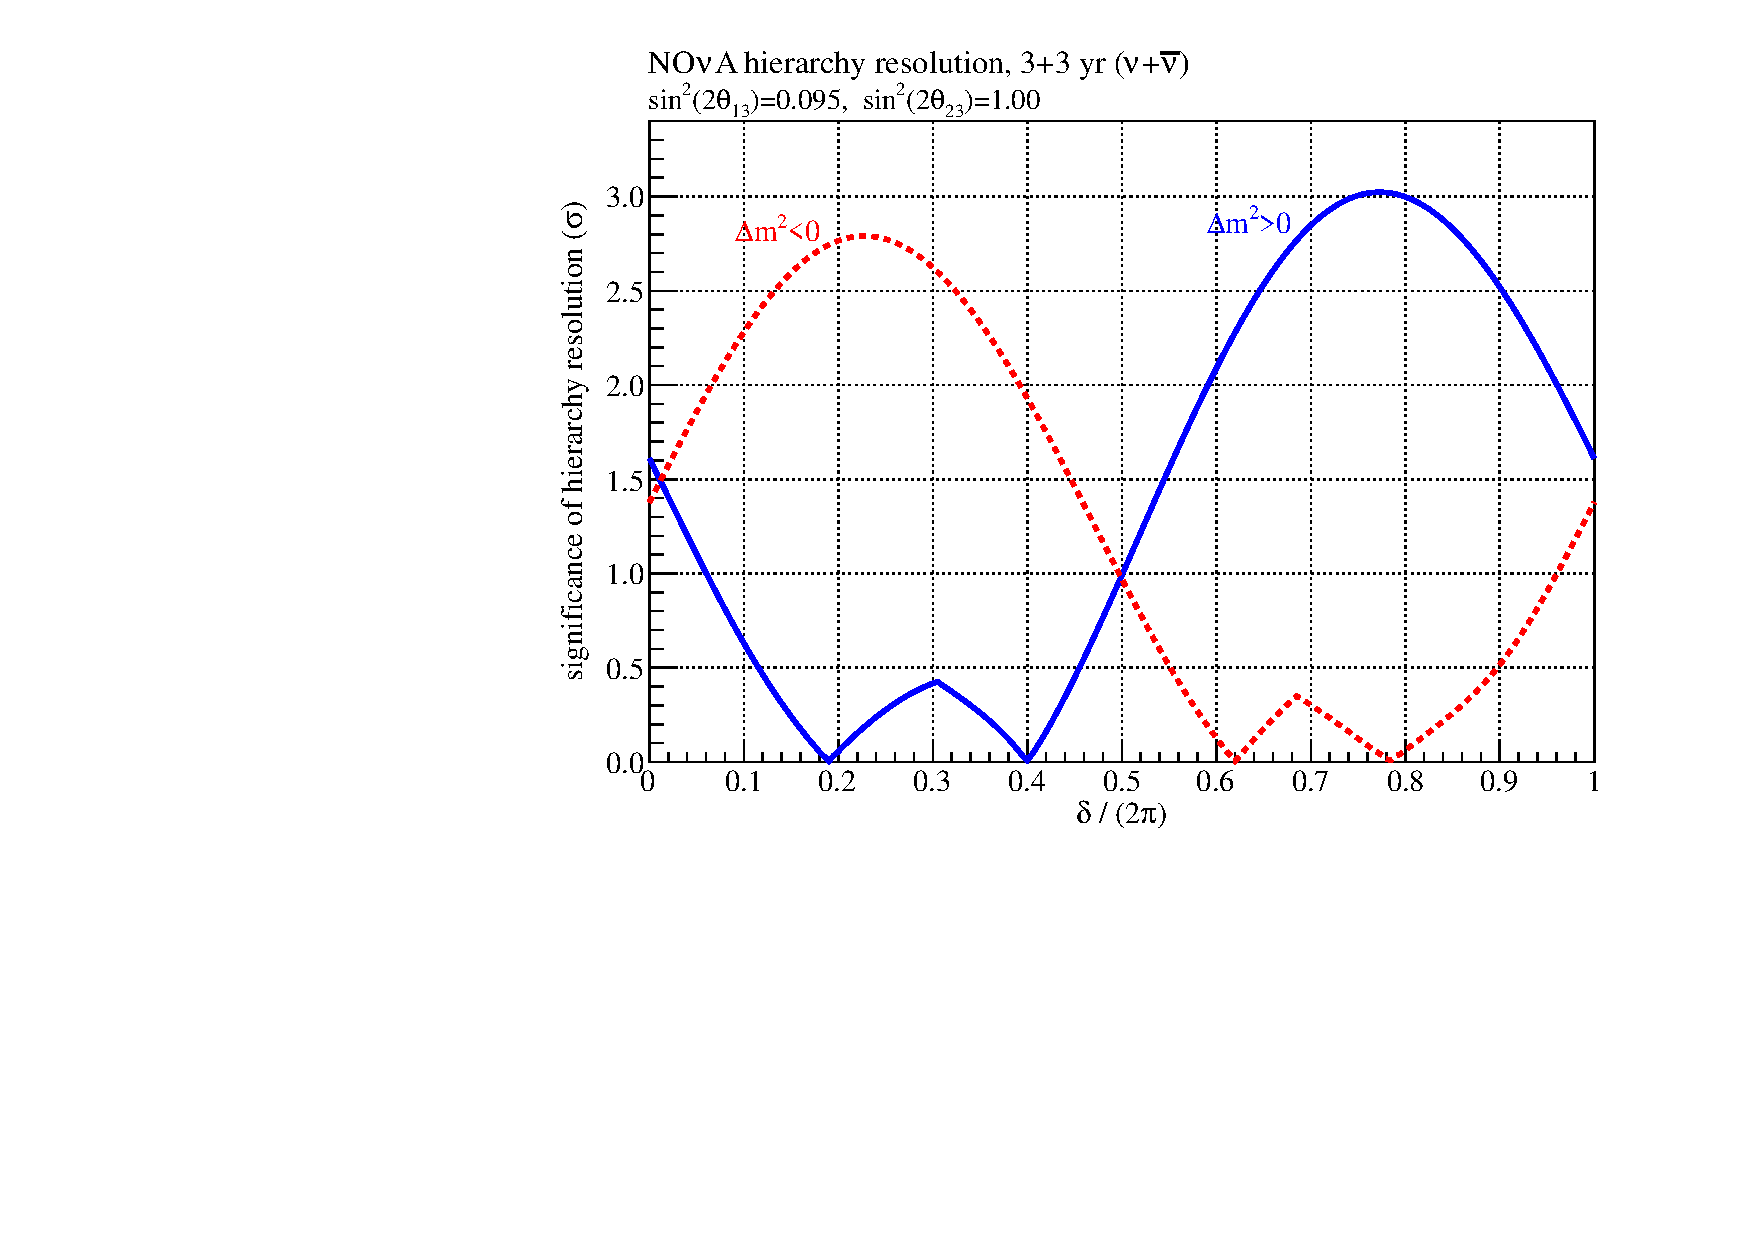
\includegraphics[width=0.9\linewidth]{\main/Neutrino/img/50_HierarchySignificance.pdf}
%   \end{minipage}
%    \caption{
%NOVA sensitivity to $\delta_{CP}$ (left) and to the mass ordering (right) as a function of  $\delta_{CP}$ with $36\times10^{20}$~POT~\cite{messier2016}. The blue solid (red dashed) curve shows the sensitivity assuming normal (inverted) mass ordering. 
%}
%\label{fig:novasensidcp}
%\end{figure}

\subsection{Future Long-baseline experiments}

While the measurements with the existing facilities continue to provide a very important contribution to the field, only for favourable parameters values will the statistical significance of the measurements of the CP violation and mass ordering exceed the 3\,$\sigma$ level. An almost complete and reasonably precise coverage of the parameter space will be provided by the next generation of experiments, Deep Underground Neutrino Experiment (DUNE) in USA and Hyper-Kamiokande in Japan. 

The 2013 strategy recommended that ``CERN should develop a neutrino programme to pave the way for a substantial European role in future long-baseline
experiments.'' This recommendation took the form of the CERN Neutrino Platform (NP) that has rapidly become the hub for neutrino physicists to develop innovative detectors for the next generation long and short-baseline experiments in USA and Japan, and beyond.

Among the most successful realizations of the CERN NP are the ProtoDUNE-SP (NP04) and ProtoDUNE-DP (NP02) that demonstrated the feasibility of very large liquid argon TPC. The NP is involved in the Japanese program with the Baby-MIND detector for J-PARC, the ongoing upgrade of the T2K Near Detector ND280 (NP07)~\cite{Abe:2019whr} and supports several other detector R\&D relevant for the next generation neutrino experiments.
A next phase of the Neutrino Platform has been recently approved, including most notably a second campaign of test beam for the ProtoDUNEs until 2021.

There is a wide support of the neutrino community at large, as shown by the recent Neutrino Town Meeting in 2018 and its conclusions~[ID45],    %\cite{townmeeting-esppu}, 
to focus on the long baseline experiments in the US and Japan. Europe should
continue to provide a balanced support for DUNE and Hyper-Kamiokande, to secure the determination of the remaining unknowns in neutrino oscillations, aim at the determination of CP violation and test the three-neutrino framework. 

The DUNE experiment [ID126] %\cite{soldner-esppu} 
is a top priority of the US High Energy Physics program. It is based on the Fermilab LBNF wide-band beam with an initial beam power of 1.2 MW of 120 GeV protons. The DUNE far detector will consist of four similar liquid argon TPCs, each with 10 kt fiducial mass, placed in the Sanford Laboratory in South Dakota, 1300 km away from Fermilab.
This detection technique will provide "bubble-chamber"-like quality data.
Large prototypes of these detectors, using the Single Phase (SP, wire chambers in the liquid argon) and Double Phase (DP, gas amplification in gaseous argon on top of the liquid argon) have been built at CERN: the ProtoDUNE-SP and ProtoDUNE-DP.
These projects have been carried out in the framework of the CERN Neutrino Platform which offered crucial support to these developments where European teams played a major role.
ProtoDUNE-SP has been exposed to a charged particle beam and has demonstrated performance exceeding the design values. %It has reached an argon purity of xx ppt, S/N of yy and has successfully operated all the High Voltages for the drift field and the wire chambers.
The construction of ProtoDUNE-DP has been completed and it will be tested with cosmic rays in the second half of 2019.
In Homestake the excavation of the main cavern hosting the DUNE far detectors has started in 2017, and the next major milestones are the installation of the first Far Detector in 2022 and the beam readiness for operation in 2026. %A sophisticated suite of near detectors, comprising a liquid argon TPC and various magnetized detectors will complete the experimental setup and give good characterization of the neutrino interaction rates.

Thanks to the very long baseline in DUNE, the matter effects will have a strong impact on the $\nu_{\mu} \rightarrow \nu_e$ appearance probability in the far detector, providing a complete coverage of the mass ordering with $\sqrt{\Delta \chi^2} > 5 $ \footnote{For the case of the mass ordering determination, the usual association of this test statistic with a $\chi^2$ distribution for one degree
of freedom is not strictly correct and its interpretation 
in terms of number of $\sigma$ of a Gaussian probability density
is not exact. This applies also to the other experiments sensitive to the mass ordering.}, and DUNE will provide a 5\,$\sigma$ measurement of CP violation for 50 \% of all $\delta_{CP}$ values (see Fig.~\ref{fig:dunesensi}). 


\begin{figure} [htbp!]
\begin{center}
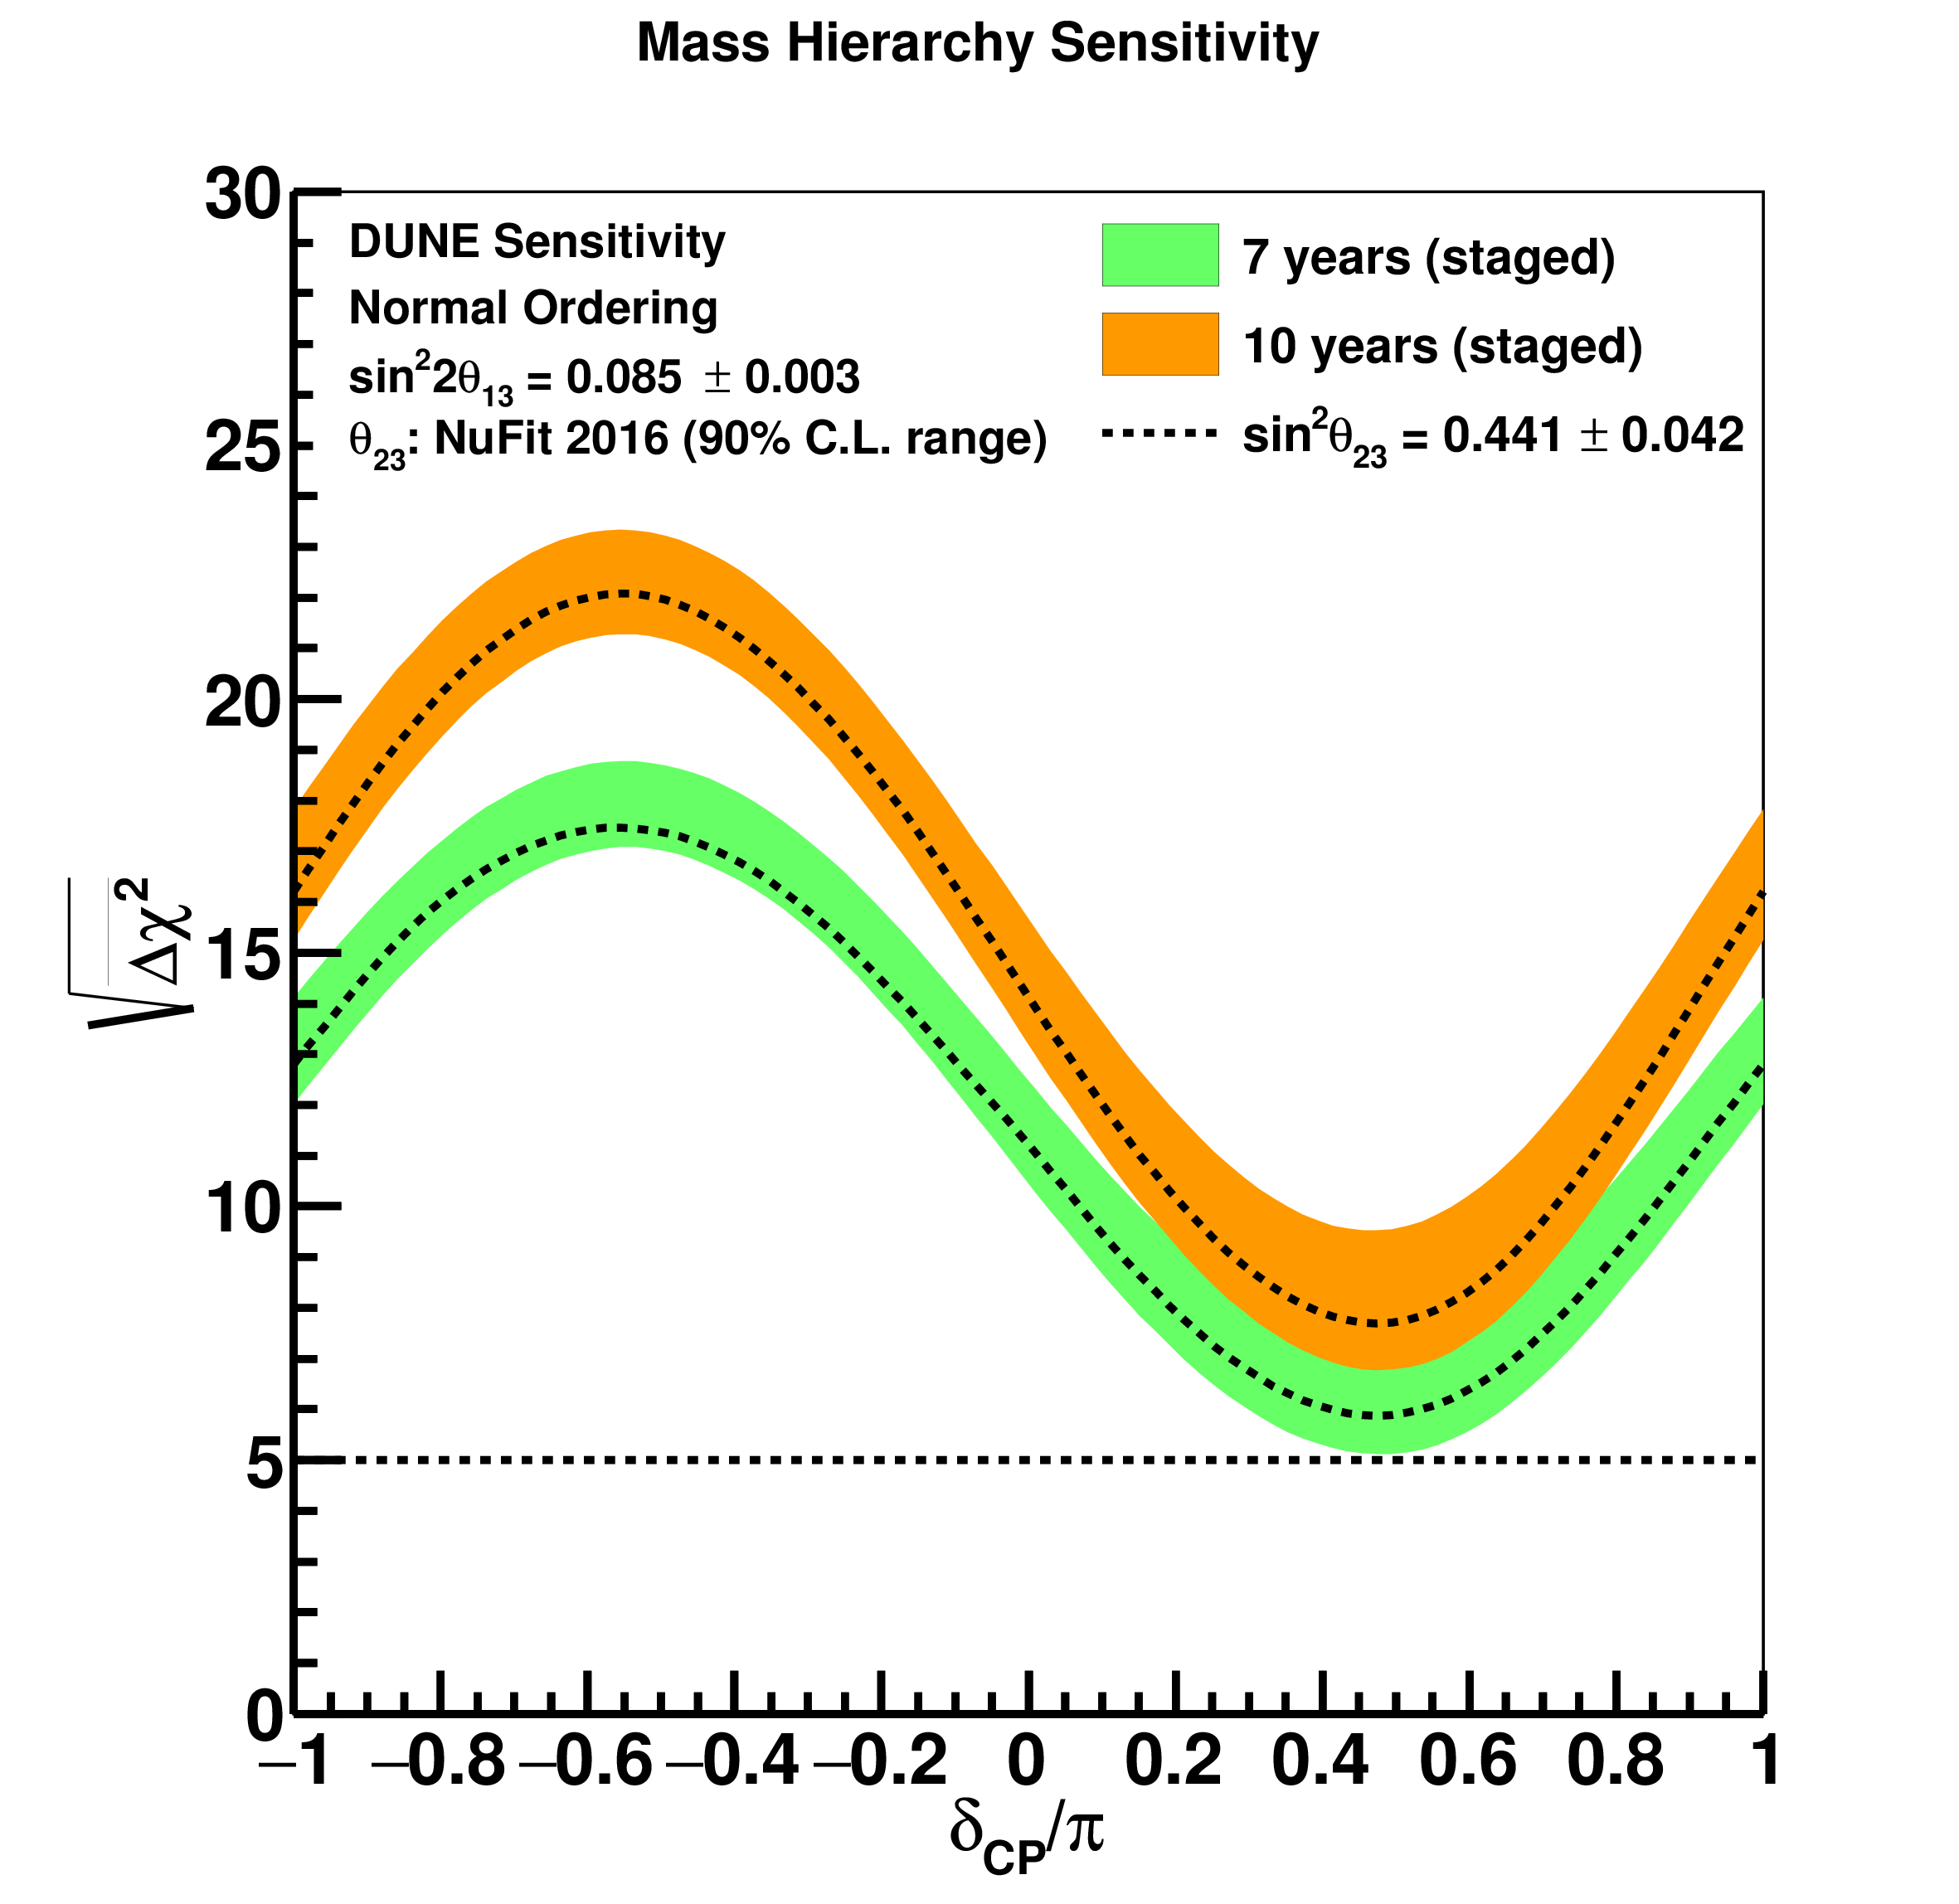
\includegraphics[width=10cm]{\main/Neutrino/img/mh_two_exps_th23band_no_2017.png}
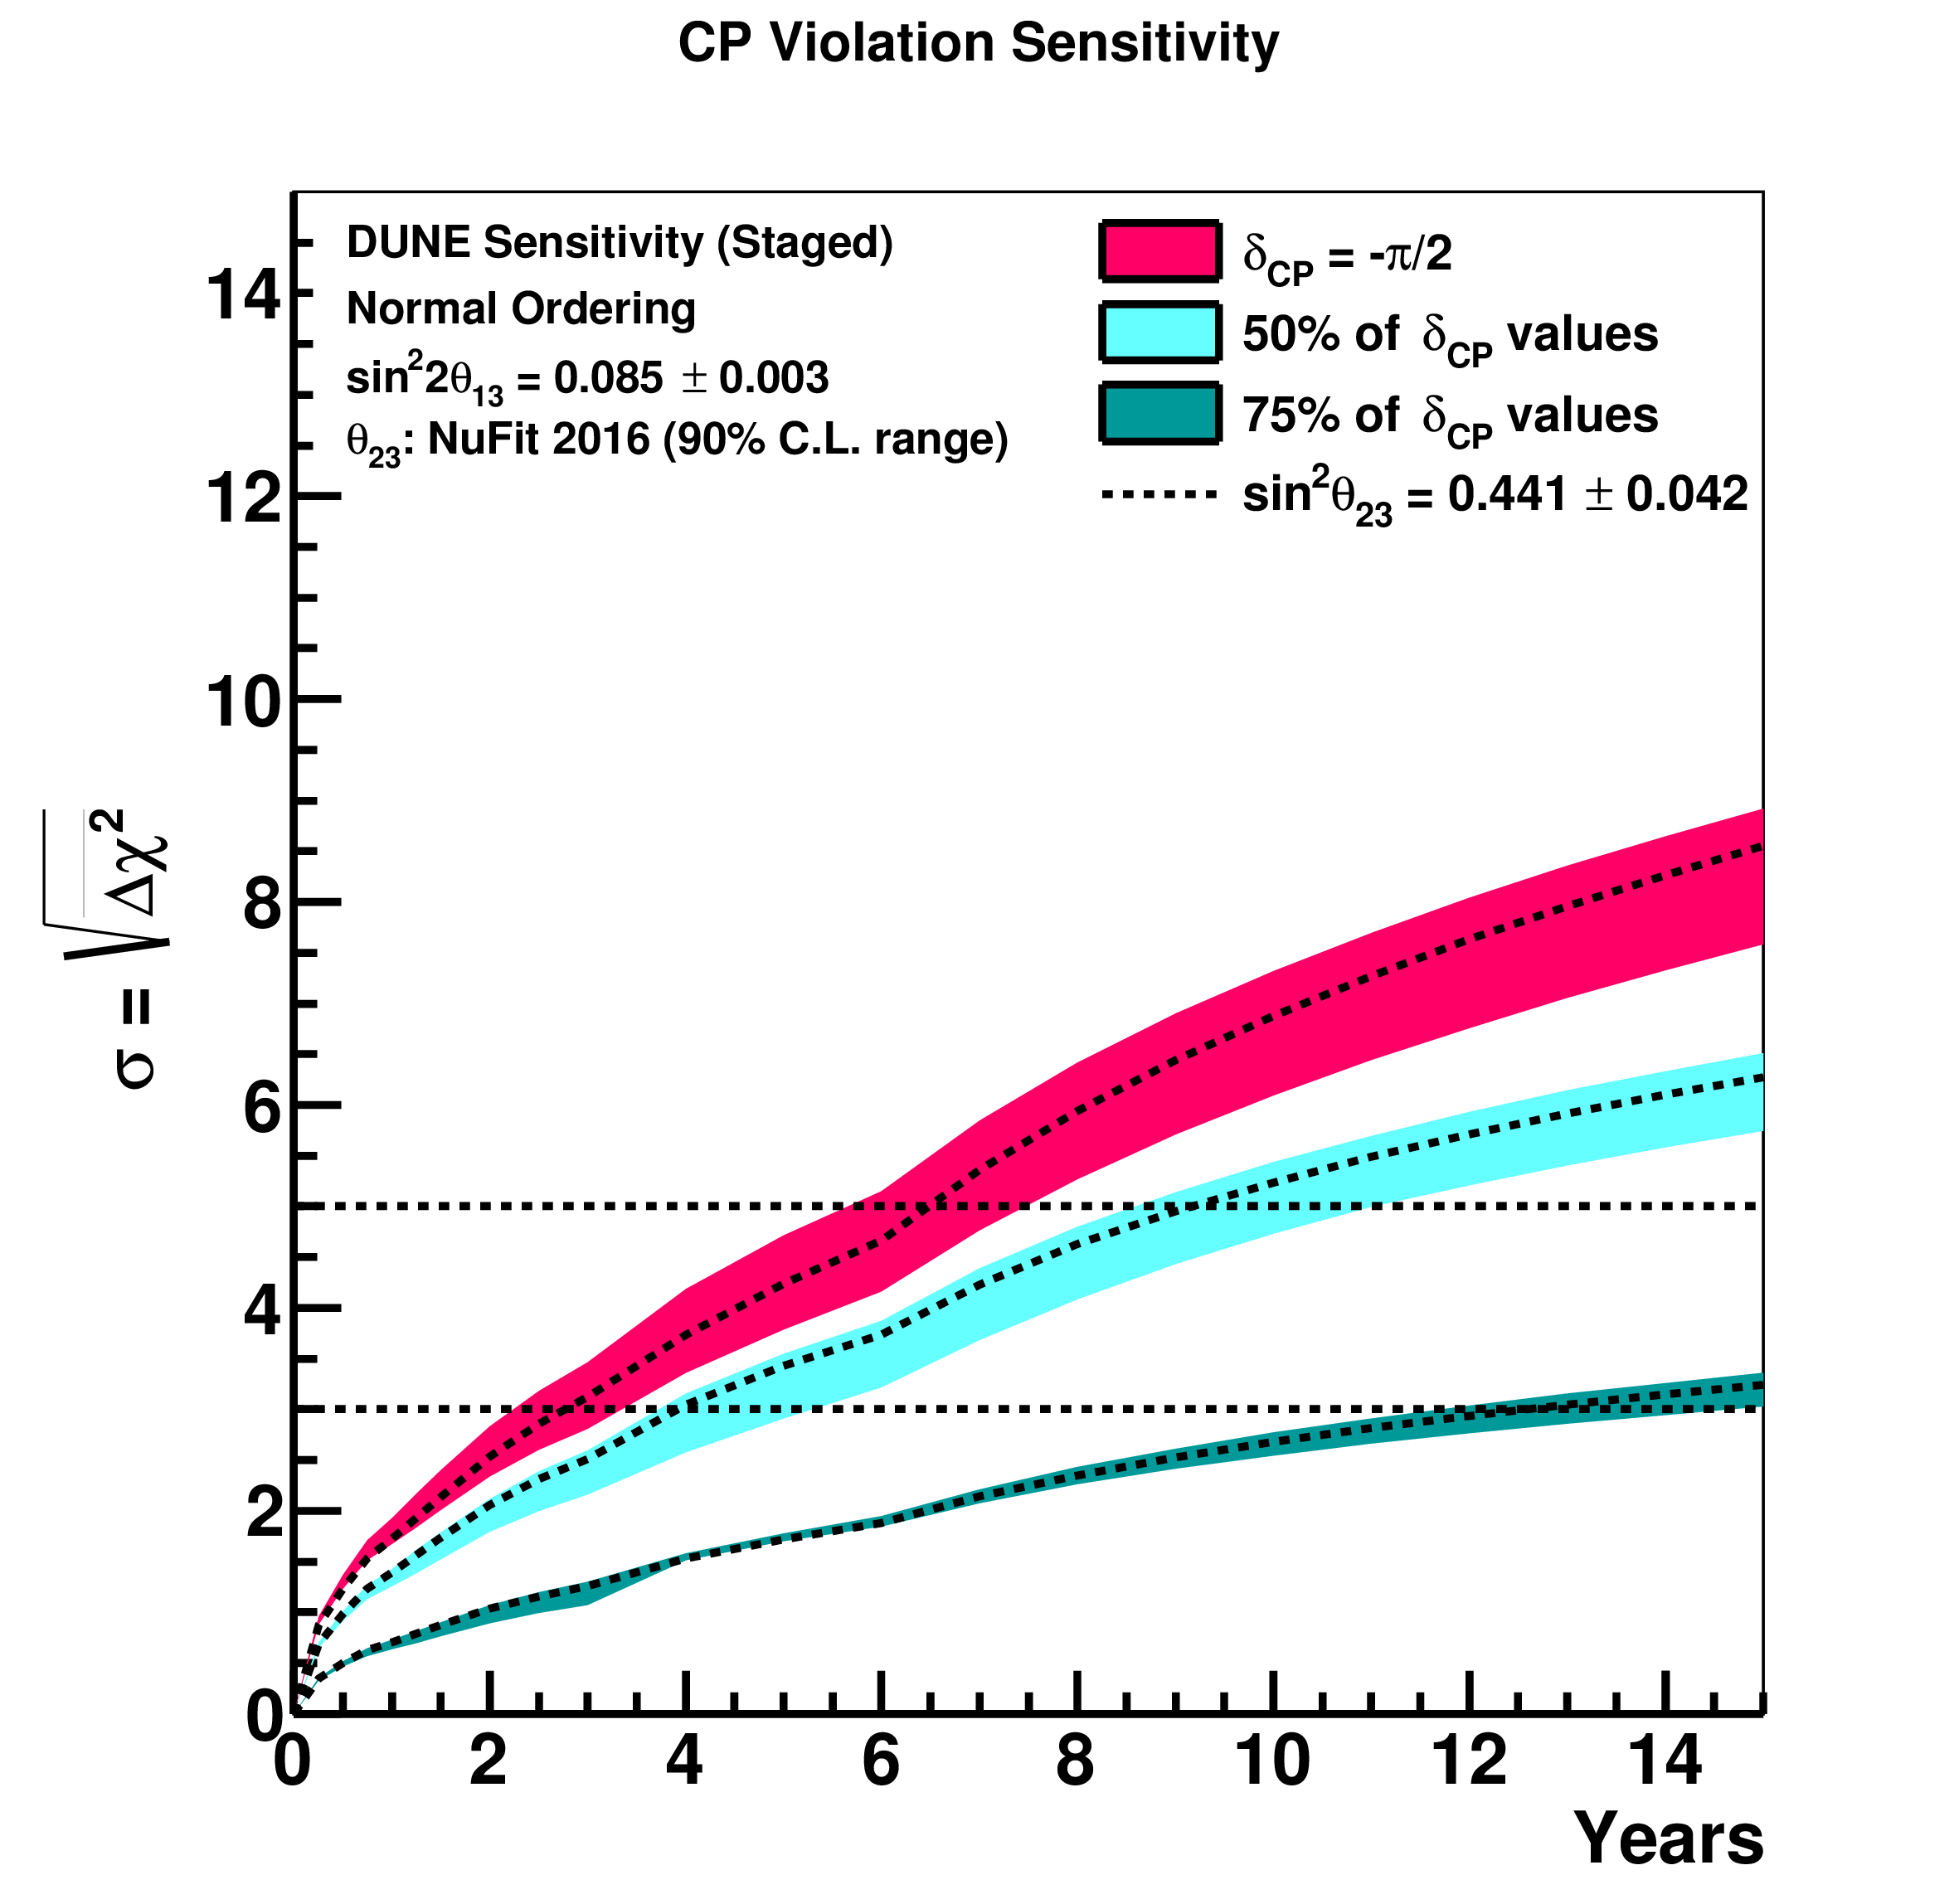
\includegraphics[width=10cm]{\main/Neutrino/img/cpv_exp_staging_th23band_2017.png}
\caption{\label{fig:dunesensi} Top: DUNE expected sensitivity~\cite{Abi:2018dnh} to the mass ordering (shown as the 
the square root of the mass ordering discrimination metric $\sqrt{\Delta \chi^2}$)
\ as a function of $\delta_{CP}$ for an exposure of 7 and 10 years. The exposure for 7 (10) years in a staged scenario is equivalent to 336 (624) kt $\times$ MW $\times$ years.
Bottom:  
the significance with which CP violation can be determined by DUNE for 75\% and 50\% of $\delta_{CP}$ values
and for $\delta_{CP}=-\pi/2 $.
}
\end{center}
\end{figure}


The Hyper-Kamiokande collaboration [ID158]  
%~\cite{lodovico-esppu} 
has been recently established and the pro-ject has been selected in 2017 by the Science Council of Japan for its Master Plan. The detector based on the well-established water Cherenkov technique will have a fiducial mass of 187 kt for one tank, located in the Gifu prefecture close to the Super-Kamiokande site (baseline 295 km). 
The target date is to complete the detector construction by 2026.
There are plans for a second similar tank, possibly located in South Korea, at a different baseline of about 1000 km. %With its mass Hyper-Kamiokande will be the largest underground detector, thereby opening new perspective for astroparticle physics as mentioned later. 
Concerning the long baseline physics program the experiment sensitivity allows the establishment of CP violation in neutrino oscillations at 5\,$\sigma$ significance for 50 \% of the allowed phase-space (Fig.~\ref{fig:hkcpv}) for an exposure of 10 years. The neutrino mass ordering can be investigated either with the addition of a second tank at a longer baseline or using the atmospheric neutrino sample.

\begin{figure} [htbp!]
\begin{center}
%add plot!!!
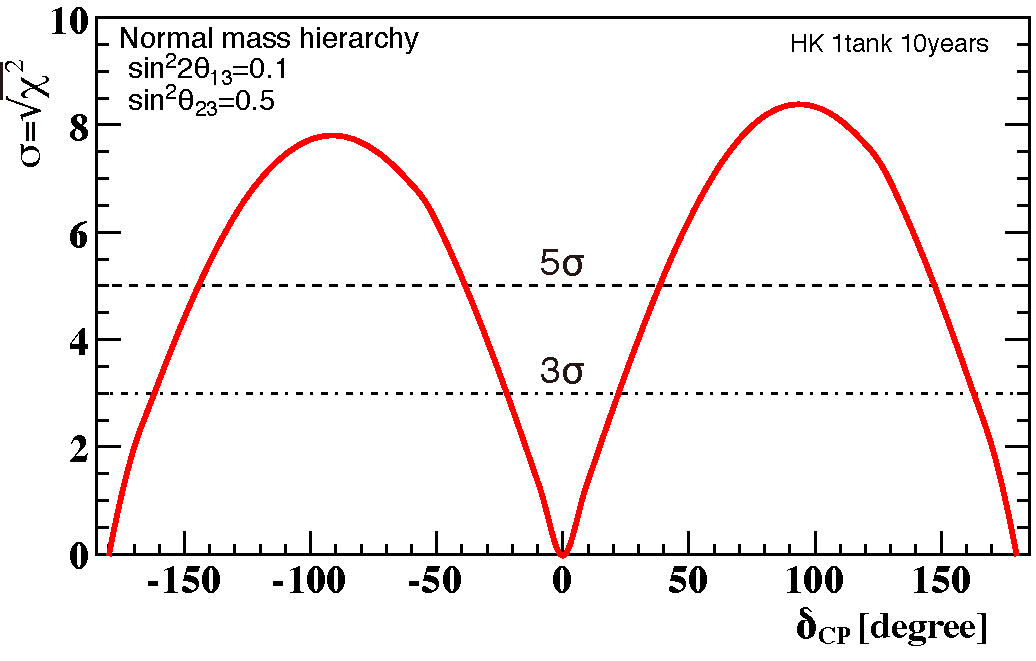
\includegraphics[width=14cm]{\main/Neutrino/img/CPresolvedSigmaVStruedCP_NH-1tank.pdf}
\caption{\label{fig:hkcpv} 
Hyper-Kamiokande expected significance to exclude $\sin \delta_{CP} = 0 $  in case of normal hierarchy~\cite{Abe:2018uyc} for an exposure of 10 years. The mass ordering is
assumed to be known. }
\end{center}
\end{figure}


The sensitivities of DUNE and Hyper-Kamiokande regarding the possible discovery of leptonic CP violation and other precision oscillation measurements are quite similar.
Nevertheless, given the pivotal importance of systematic uncertainties in these measurements, the
availability of two experiments with orthogonal choices regarding beam design, detector technology
and baseline will be essential for reaching authoritative conclusions~\cite{Cao:2015ita}.
The complementarity between DUNE and Hyper-Kamiokande becomes even more evident for tests of new
physics scenarios: because their relative sensitivities to the standard 3-family oscillation and to
non-standard scenarios, such as e.g. a new type of neutrino matter effects~\cite{Liao:2016orc}, are different, their
combination will allows to probe and characterize new physics effects more comprehensively.
Finally, DUNE and HyperK are highly complementary in their physics program beyond
accelerator-based neutrinos.



DUNE and Hyper-Kamiokande, as well as JUNO, that will be described below, will also be the largest and more sophisticated neutrino detectors underground, offering sensitivity to a range of exotic and astrophysical process among which:
the search for proton decay, the study of neutrinos produced by core-collapse supernovae (CCSN), and new studies of solar and atmospheric neutrinos. 
Proton decay is a generic prediction of Grand Unification Theories. The current best limit  at 10$^{34}$ years has been established by Super-Kamiokande~\cite{Miura:2016krn}. DUNE and Hyper-Kamiokande have the sensitivity to increase this limit by an order of magnitude. 
%will extend this to 10$^{35}$  years and conduct high sensitivity searches also for other decay modes.

The observation of 25 neutrinos emitted by SN1987A has marked the birth of neutrino  and multimessenger astrophysics, as detailed in chapter~\ref{chap:cosm}. DUNE, Hyper-Kamiokande and JUNO will be excellent detectors of the neutrinos produced by the next CCSN in our galaxy, providing complementary samples of several 10$^4$ events and  allowing to follow the time development of neutrino emission during the collapse and rebound phases to better understand the still largely unknown physics of these spectacular stellar collapses. 
Hyper-Kamiokande will provide the largest sample due to its large mass, with event-by-event determination of the energy down to 3 MeV. It will mainly detect anti-electron neutrinos using the inverse beta decay reaction. In addition it can provide a 1 degree pointing accuracy for a supernova at 10 kpc, enabling multi-messenger studies. On the other hand DUNE will detect electron neutrinos via $\nu_e + {}^{40} Ar \rightarrow e^- + {}^{40} K^*$. This is particularly interesting because the supernova neutrino emission begins with the neutronization burst, an initial sharp, bright flash of $\nu_e$  from $ p + e \rightarrow  n + \nu_e$.

The European Spallation Source in Lund (Sweden) will provide a 5 MW proton beam. It has been proposed to use this facility to provide a neutrino beam for long baseline studies in Europe [ID98] %\cite{ekelof-esppu}. 
with a far detector located at the second oscillation maximum, where CP violation effects are stronger. At the moment this project is in its design phase. In the best case this facility would start several years after the DUNE and Hyper-Kamiokande experiments and would not provide a significantly superior sensitivity to measure the PMNS phase $\delta_{CP}$. However, ESS could be an important test-bed for R\&D on new intense neutrino beams along the road towards a Neutrino Factory. 
Indeed if, for instance, $\delta_{CP}$ is close to $\pm \pi/2$  or if
$ \sin \delta_{CP} $ is close to 0, improved precision
with respect to DUNE and Hyper-Kamiokande should be considered.
A Neutrino Factory~\cite{Bogomilov:2014koa}, where the neutrinos are produced by the decay of muons in a storage ring, would be the natural next to next step for long baseline experiments beyond DUNE and Hyper-Kamiokande. It would be a unique facility to reach a precision of $6^{\circ}$ on the measurement of $\delta_{CP}$.

\subsection{ Future experiments with reactor and atmospheric neutrinos to determine the mass ordering}

The study of the neutrino mass ordering has spurred many new ideas since the discovery of the last mixing angle $\theta_{13}$. As $\theta_{13}$ is relatively large, several non-leading effects are within experimental reach and could allow to establish the mass ordering with new methods.

The Jiangmen Underground Neutrino Observatory (JUNO)~[ID10] %\cite{juno-esppu}
collaboration is building underground a large liquid scintillator detector, with a mass of 20 kt. It is located in China, at a distance of 53 km from two clusters of nuclear reactors. One of the main goals of JUNO is the detection of antineutrinos from these reactors. At these distances the electron neutrino survival probability will be  
modulated by $\Delta m^2_{21}$, with slow oscillations, on which a term governed by $ \Delta m^2_{31}$ will superimpose much faster oscillations with a much smaller amplitude. The latter carry information about the mass ordering. In order to do this, an unprecedented 3\%/$\sqrt{E}$ energy resolution has to be reached, which is an experimental challenge.
The measurement of antineutrino spectrum with excellent energy resolution will also lead to the precise determination of the neutrino oscillation parameters $\sin^2 \theta_{12}$, $\Delta m^2_{12}$, and $|\Delta m^2_{ee} |$ ($ \Delta m^2_{ee}= \cos^2 \theta_{12}  \Delta m^2_{31}  + \sin^2 \theta_{12}  \Delta m^2_{32} $) to an accuracy of
better than 1\%. JUNO will start taking data in 2021.

Another approach for the study of neutrino oscillations is to use atmospheric neutrinos. These are produced by the decay of pions created in high energy cosmic ray interaction in the atmosphere. The advantage of this neutrino source is its range in energy (typically from sub GeV to hundreds of GeV) and in oscillation length, reaching 12000 km.
The disadvantage is that this source contains both neutrinos and anti-neutrinos, $\nu_\mu$ and $\nu_e$. Since the large Cherenkov detectors used to detect these neutrinos can not differentiate between neutrinos and antineutrinos, matter effects are convoluted with flux and cross-section effects. 
%This smearing reduces the sensitivity to the mass ordering. 
Moreover, the critical energy region to carry out this measurement is in the few GeV range, which is difficult to attain with a sparse detector array. Nevertheless, the IceCube experiment has shown a good sensitivity to the $\nu_\mu$ disappearance. The ORCA experiment~[ID84] %\cite{appec-esppu} 
 is part of the KM3NeT project and foresees to deploy an array of instrumented lines in the Mediterrenean, close to Toulon (France), with a distance between PMT of about 10m. Sensitivity studies show that this detector might provide a 3 $\sigma$ measurement of the mass ordering after 3 years of data-taking. The detector construction has started and the target date for its completion is 2024. A new neutrino beam from Protvino (Moscow) to ORCA has been proposed [ID124] with a baseline of 2595 km. The detector configuration, the performance and the physics case need to be established and studied in more details.


\subsection{ Precision flux and cross-section measurements}


A crucial point for the overall neutrino program is the precision knowledge of neutrino fluxes and cross-sections. Indeed, as the modulation of the $\nu_\mu \rightarrow \nu_e$ appearance probability induced by the PMNS $\delta_{CP}$ phase is about 30 \% on the first oscillation maximum, the precision extraction of oscillation parameters requires good control of the interaction rates, at the percent level, to be compared to the current level of 5-7 \% reached for instance by T2K.

This impressive reduction of the systematic uncertainties requires a full-fledged program to develop new techniques and detectors, innovative measurements and phenomenological models. Europe, and CERN in particular, could play a crucial role in implementing this program on the basis of the present expertise, and of existing or new facilities.
In the following we will briefly sketch some important developments along this road.

The neutrino beams used in long baseline experiments rely on the production of hadrons by impinging a primary proton beam on a target. The precise knowledge of the hadroproduction cross-section is a crucial ingredient to improve the precision on the neutrino fluxes. Europe has a unique facility with the CERN NA61/SHINE experiment~[ID13] %\cite{na61-esppu} 
at the SPS, capable of large acceptance and high resolution, that has already produced several crucial measurements for T2K. It plans to upgrade its detector and to continue its program of measurements with replica targets for the DUNE and Hyper-Kamiokande experiments. %Moreover, the measurements by NA61 can also improve the knowledge on the flux of atmospheric neutrinos.

The ENUBET (NP06)~[ID57] %\cite{enubet-esppu} 
collaboration  proposes a dedicated facility to precisely measure the $\nu_\mu$ and $\nu_e$ cross-section improving by an order of magnitude over the present knowledge. They propose to do so with a combination of narrow-band neutrino beams and monitored beams, instrumenting the decay tunnel with a segmented calorimeter. 


The $\nu$STORM~[ID154] %\cite{nustorm-esppu} 
collaboration proposes a new facility capable of delivering a precisely (1\%) known neutrino beam. It relies on a new concept, where the neutrinos are produced in a storage ring by the decay of muons. Besides precise neutrino nucleus cross-sections useful for DUNE and Hyper-Kamiokande, the $\nu$STORM facility can also be used for searches for sterile neutrinos beyond the capabilities of the Fermilab short baseline experiments and can also serve as the test facility for the development of  a neutrino factory and muon accelerators
towards a multi-TeV lepton-antilepton collider. The operation of ENUBET and/or $\nu$STORM by 2027 would maximize the impact of these measurements for the world neutrino program. A study should be set-up to evaluate the possible implementation, performance and impact
of a percent-level electron and muon neutrino cross-section measurement facility (based on e.g. ENUBET or $\nu$STORM) with conclusion in a few years.

Together with these developments aimed at precisely known neutrino flux and cross-sections, a corresponding development plan is unfolding for high precision near-detectors [ID106, ID131]~\cite{Abe:2019whr} %\cite{Bordoni-esppu, petti-esppu}
and for the development of precise and reliable neutrino interactions models~\cite{Alvarez-Ruso:2017oui}. The latter point will require a close collaboration and much increased effort between neutrino physicists, nuclear physicists and phenomenologists, where Europe is today playing a leading role and can continue to do so in the future provided this fragile community receives the much needed support.


%ESSNUSB Nufact (Protvino to Orca ?)

%Supporting program: NA61 xsec neutrino platform ND Nustorm Enubet

%Future developments (nufactory) Nustorm
